\begin{figure}
    \centering
    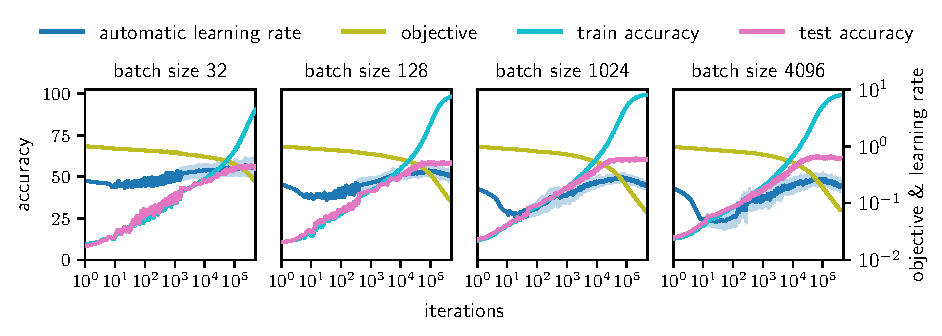
\includegraphics[width=\textwidth]{figures/pdf/plot4}
    \caption{\captiontitle{Benchmarking automatic gradient descent at varying mini-batch size.} We trained four-layer fully-connected networks on CIFAR-10. The mini-batch size ranged from 32 to 4096. Test accuracy generally improved with increasing mini-batch size: the final test accuracies, in order of increasing mini-batch size, were 55.0\%, 58.0\%, 60.0\% and 59.8\%. The automatic learning rate seemed to initially dip, and this effect was more pronounced for larger mini-batch sizes. Metrics were computed every iteration during the first epoch and once per epoch from thereon---this explains the kinks visible in the plots.
    } \label{fig:4}
\end{figure}